\documentclass[10pt,twocolumn]{article}
\usepackage[margin=0.75in]{geometry}
\usepackage[T1]{fontenc}
\usepackage[utf8]{inputenc}
\usepackage{amsmath,amssymb,amsfonts}
\usepackage{booktabs,array,url,graphicx}
\usepackage[hidelinks]{hyperref}
\usepackage{cite}

\def\UrlBreaks{\do\/\do-\do\_}

\title{\textbf{\Large Beyond the Verification Mirage: Source-Bound Execution Provenance and Dynamic KV-Cache Precision Management for Autonomous Gemma~4 Coding Agents}\\[0.8ex]
\large A Dual-Integrity Architecture for External Execution Provenance and Bidirectional KV-Cache Precision Scaling in Edge and Cloud Coding Agents}

\author{\textbf{Manimaran K.}\\
\textit{Google -- The Gemma 4 Developer Agent Competition (Paper Track)}}
\date{}

\begin{document}

\maketitle

\begin{abstract}
Deploying open-weight Gemma~4 models (\texttt{gemma-4-31b-it-qat-w4a16-ct}, \texttt{e4b}, \texttt{e2b}) as autonomous software engineering agents across competition sandboxes and mobile edge devices reveals two coupled failure modes: \textit{The Verification Mirage} and \textit{Attention Dilution with Context Exhaustion}. In air-gapped sandboxes, test runners frequently import pre-installed libraries from global \texttt{site-packages} rather than the mutated workspace checkout, generating false acceptances (unfixed code passing) and false rejections (valid patches evaluated against stale binaries). Concurrently, expansive multi-file diagnostic loops flood context windows past 23,000 tokens, diluting attention over root causes and triggering Over-Editing Syndrome while exhausting edge RAM. We present a dual-integrity architecture bridging external execution provenance with internal KV-cache precision management. First, \textit{Check-Process Provenance Receipts} cryptographically bind module origin (\texttt{\_\_file\_\_}), workspace SHA-256 digests, and assertion results within an atomic child process across a four-state evidence taxonomy ($S_1 \dots S_4$). Second, \textit{Traceback Anchoring} leverages call-graph and abstract syntax tree (AST) traversal to bound context reads to 30--50 line frames. Third, \textit{FluxKV} introduces a non-monotonic KV-cache lifecycle ($\text{FP16} \leftrightarrow \text{INT4} \leftrightarrow \text{INT2}$) with low-rank residual sketches, dynamically compressing transient bash logs while restoring FP16 fidelity to early code definitions when attention velocity shifts back during patch synthesis. Across 4 benchmark repositories (\texttt{requests}, \texttt{fastapi}, \texttt{rich}, \texttt{httpx}), an $N=32$ replication of a 16-condition matrix, live Kaggle $4\times$ NVIDIA L4 evaluations, and Android edge execution under 3,107~MiB PSS contention, our framework eliminates 100\% of false source claims ($8/16 \to 0/16$), preserves a 0.17 solve rate where multi-file search degrades to 0.10, and reduces KV-cache memory by $3.90\times$ steady-state (up to $4.7\times$ peak dynamic reduction) with 15.2\% lower reconstruction loss and 100\% needle retrieval accuracy.
\end{abstract}

\section{Introduction \& Problem Formulation}

Autonomous software engineering agents powered by modern open-weight large language models (LLMs), such as the Gemma~4 family~\cite{gemma2024}, operate through iterative interaction loops: reading repository structures, formulating bug hypotheses, applying localized file edits, and executing test suites~\cite{jimenez2024swebench,yang2024sweagent,xia2024agentless}. In cloud competition sandboxes and mobile edge deployments, agents are expected to independently locate root causes across complex multi-file repositories, synthesize patches, and verify functional correctness against regression suites. However, rigorous empirical examination across 120 experimental slots in 10 development studies and live Kaggle leaderboard submissions reveals that standard agentic loops suffer from a critical dual-integrity breakdown: external execution isolation failures coupled with internal attention dilution and memory contention.

\subsection{The Verification Mirage}
In offline competition sandboxes and continuous integration environments, containers are air-gapped and pre-populated with standard libraries to accelerate evaluation runs. When an agent edits a source file within a checked-out repository $\mathcal{W}$, invoking test commands (such as \texttt{pytest} or \texttt{python3 -c}) frequently resolves imports from global system paths (such as \texttt{/usr/local/lib/python3.x/site-packages/}) rather than the active workspace $\mathcal{W}$. This occurs because Python's module resolution algorithm (\texttt{sys.path} and \texttt{sys.meta\_path} PathFinder) defaults to pre-installed wheels unless explicit editable links (\texttt{pip install -e .}) or strict environment overrides are configured.

Furthermore, Python's runtime caches loaded module objects in the global dictionary \texttt{sys.modules}. When a test runner executes a preflight diagnostic or collects test definitions, modules imported from \texttt{site-packages} remain permanently cached in memory. Subsequent file edits applied to $\mathcal{W}$ on disk are completely ignored by the running Python process because the runtime reuses the stale module reference. Standard mitigation strategies, such as invoking \texttt{importlib.reload()}, fail catastrophically in production codebases due to circular package dependencies, sub-module binding desynchronization, and persistent class instances holding references to old type objects.

In air-gapped evaluation environments where dynamic package compilation is disabled, this decoupling creates the \textit{Verification Mirage}:
\begin{enumerate}
    \item \textbf{False Acceptance}: The model introduces an invalid syntax edit or an empty no-op, yet test assertions pass because the runner executes against the untouched, working pre-installed wheel.
    \item \textbf{False Rejection}: The model generates a semantically correct patch in $\mathcal{W}$, but tests fail because the runner executes against the unpatched, buggy system library.
\end{enumerate}
Crucially, separate preflight checks (verifying source paths prior to running tests) fail to resolve this vulnerability. Subprocess invocations, shell environment shifts, virtual environment activation scripts, and test runner plugins frequently reset \texttt{sys.path}, decoupling preflight guarantees from the actual test assertions.

\subsection{The Edge Silent No-Op \texorpdfstring{($S_1$)}{(S1)}}
When deploying compact models such as Gemma~4 E2B on physical edge devices (e.g., Samsung Galaxy S24 FE via LiteRT-LM CPU) alongside concurrent background applications, memory pressure escalates dramatically. The mobile operating system enforces strict memory governance via the low-memory killer daemon (\texttt{lmkd}) and Dynamic Thermal Management. Under heavy memory contention exceeding 3,100~MiB Proportional Set Size (PSS) and elevated thermal envelopes (40.9$^\circ$C), agents frequently terminate with shell exit code 0 and report \texttt{loop\_succeeded=true} without emitting any concrete file edits ($\Delta_{\text{git}}(\mathcal{W}) = \emptyset$).

This occurs because internal execution timeouts and caught memory allocation exceptions cause the agent loop to abort gracefully before patch emission. Conventional benchmarks that evaluate success based on clean process exit codes blindly record these instances as valid executions, masking severe degradation in edge agent reliability under realistic operating conditions.

\subsection{Attention Dilution \& Over-Editing Syndrome}
Standard coding agents attempt to resolve bugs by issuing broad search queries (\texttt{grep}, \texttt{find}, multi-file recursive reads). This strategy rapidly floods the context window with thousands of tokens of irrelevant source files, fixture boilerplate, and foreign traceback logs. In deep multi-turn interactions exceeding 23,000 tokens, softmax attention mass over the true defect site decays exponentially.

Under Rotary Position Embeddings (RoPE), when context length scales into tens of thousands of tokens, query-key dot products in intermediate transformer layers suffer from dispersion across irrelevant background tokens. In response, Gemma~4 31B agents exhibit \textit{Over-Editing Syndrome}: experiencing high uncertainty over localized defect boundaries, the model initiates speculative "shotgun debugging." It hallucinates modifications across dozens of untouched caller files, breaking downstream interfaces and triggering circular dependencies. On the live Kaggle competition leaderboard, expanding agent exploration from single-file scope to multi-file exploration caused resolve rates to plummet by an exact 40.0\% relative drop (from 10 down to 6 solved tasks, 0.17 to 0.10).

\subsection{Contributions}
We formulate a unified dual-integrity systems architecture resolving both environmental and internal memory degradation:
\begin{enumerate}
    \item \textbf{Check-Process Provenance Receipts}: An atomic child-process execution primitive that cryptographically certifies module provenance, file content hashes, and test assertions in a unified payload across a four-state evidence taxonomy ($S_1 \dots S_4$).
    \item \textbf{Call-Graph \& AST Traceback Anchoring}: A graph traversal mechanism that navigates execution call-graphs and AST dependency subgraphs to bound context windows to 30--50 line defect frames, suppressing multi-file noise.
    \item \textbf{FluxKV Dynamic Precision Lifecycle}: A non-monotonic KV-cache manager that continuously tracks token attention velocity over the bipartite interaction graph, quantizing stale logs to INT2 while leveraging low-rank residual sketches to restore FP16 fidelity to early code definitions.
    \item \textbf{Empirical Validation}: Full qualification across 4 major repositories, 16 adversarial container conditions ($N=32$), live Kaggle 4x L4 leaderboard evaluations, mobile edge profiling, and CUDA KV-cache benchmarks, bounded by Manski partial identification intervals.
\end{enumerate}

\section{Systems Architecture \& Graph Reasoning}

The overall architecture unites external OS-level process provenance with internal model attention graph dynamics. We model the autonomous software engineering problem through three distinct graph representations: execution call-graphs, token attention graphs, and verification state machines.

\subsection{Check-Process Provenance Receipts}
To eliminate the Verification Mirage, test execution must be atomically bound to the mutated workspace. Rather than executing tests via unconstrained shell commands, our verification engine spawns an isolated child process executing an inline Python verification wrapper:
\begin{equation}
    \mathcal{R}_{\text{prov}} = \big\langle \mathcal{M}_{\text{name}}, \text{Path}(\mathcal{M}), \text{SHA256}(\mathcal{F}_{\text{target}}), \text{Result}(\mathcal{A}) \big\rangle
\end{equation}
where $\mathcal{M}$ is the imported module, $\mathcal{F}_{\text{target}}$ is the edited source file, and $\mathcal{A}$ represents the verification assertion snippet. The wrapper executes within a dedicated sub-interpreter, inspects the canonical filesystem path via \texttt{os.path.realpath(module.\_\_file\_\_)}, computes the SHA-256 cryptographic hash of $\mathcal{F}_{\text{target}}$ directly from disk, evaluates assertion $\mathcal{A}$ in an isolated namespace, and emits a structured JSON receipt across standard output.

We structure all agent trajectory outcomes into a formal four-state evidence taxonomy $\mathcal{S} = \{S_1, S_2, S_3, S_4\}$:
\begin{itemize}
    \item \textbf{State $S_1$ (Silent No-Op)}: The agent returns success (\texttt{exit\_code = 0}), but git diff inspection reveals no workspace modifications: $\Delta_{\text{git}}(\mathcal{W}) = \emptyset$.
    \item \textbf{State $S_2$ (Foreign Origin Abstention)}: Workspace edits exist ($\Delta_{\text{git}}(\mathcal{W}) \neq \emptyset$), but $\text{Path}(\mathcal{M}) \not\subset \mathcal{W}$ (resolving instead to system \texttt{site-packages}). The engine strictly abstains from claiming repair, preventing False Acceptances.
    \item \textbf{State $S_3$ (Bound Rejection)}: Module path satisfies $\text{Path}(\mathcal{M}) \subset \mathcal{W}$ and file SHA-256 matches disk state, but assertion $\mathcal{A}$ fails.
    \item \textbf{State $S_4$ (Bound Verified Repair)}: Simultaneously satisfies $\Delta_{\text{git}}(\mathcal{W}) \neq \emptyset$, $\text{Path}(\mathcal{M}) \subset \mathcal{W}$, matching SHA-256 digest, and passing assertions ($\text{Result}(\mathcal{A}) = \text{PASS}$).
\end{itemize}

\subsection{Traceback Anchoring \& Call-Graph Traversal}
To prevent Attention Dilution, we formalize repository diagnosis as graph reasoning over two directed structures: the dynamic execution call-graph $\mathcal{G}_{\text{call}} = (\mathcal{V}_{\text{frames}}, \mathcal{E}_{\text{calls}})$ and the static abstract syntax forest $\mathcal{G}_{\text{AST}} = (\mathcal{V}_{\text{nodes}}, \mathcal{E}_{\text{tree}})$. Each stack frame is a 4-tuple $v = (\text{path}(v), \text{line}(v), \text{func}(v), \text{locals}(v))$, while each AST node $u \in \mathcal{V}_{\text{nodes}}$ spans source interval $\operatorname{span}(u) = [L_{\text{start}}(u), L_{\text{end}}(u)]$ with grammar type $\operatorname{type}(u) \in \Sigma_{\text{AST}}$. Let $\Sigma_{\text{scope}} = \{\texttt{FuncDef}, \texttt{AsyncFuncDef}, \texttt{ClassDef}\} \subset \Sigma_{\text{AST}}$ denote enclosing functional scopes.

We define the formal projection operator $\pi: \mathcal{V}_{\text{frames}} \to \mathcal{P}(\mathcal{V}_{\text{nodes}})$ mapping an execution frame to its minimal enclosing functional AST subtree:
\begin{equation}
\begin{split}
    \pi(v) = \arg\min_{u \in \mathcal{V}_{\text{nodes}}} \Big\{ &|\operatorname{span}(u)| : \text{file}(u) = \text{path}(v), \\
    &\text{line}(v) \in \operatorname{span}(u), \\
    &\operatorname{type}(u) \in \Sigma_{\text{scope}} \Big\}
\end{split}
\end{equation}
where $|\operatorname{span}(u)| = L_{\text{end}}(u) - L_{\text{start}}(u) + 1$. Lifting $\pi$ across the call trace induces the graph morphism $\Pi(\mathcal{G}_{\text{call}}) = \bigcup_{v \in \mathcal{V}_{\text{frames}} \cap \mathcal{W}} \pi(v) \in \mathcal{P}(\mathcal{G}_{\text{AST}})$. When an unhandled exception occurs, our protocol executes \textit{Traceback Anchoring}:
\begin{enumerate}
    \item \textbf{Workspace Call-Graph Sink Isolation}: The agent traverses $\mathcal{G}_{\text{call}}$ starting from the exception sink to extract the terminal execution frame $v_{\text{term}} = \operatorname{Sink}(\{v \in \mathcal{V}_{\text{frames}} \mid \text{path}(v) \subset \mathcal{W}\})$, unconditionally filtering external test harness frames ($\text{path}(v) \not\subset \mathcal{W} \implies \pi(v) = \emptyset$).
    \item \textbf{AST Subtree Bounding}: Evaluating $\pi(v_{\text{term}})$ extracts a bounded target window $W_{\text{target}} = \mathcal{F}[L_{\text{start}}(\pi(v_{\text{term}})) : L_{\text{end}}(\pi(v_{\text{term}}))]$ spanning exactly 30--50 lines of the target function or class definition, ensuring surrounding helper modules remain unmodified.
    \item \textbf{Scope-Disciplined Patch Synthesis}: Context ingestion is restricted strictly to $W_{\text{target}}$, problem statement tokens, and reproduction assertion $\mathcal{A}$. Edits outside $\operatorname{span}(\pi(v_{\text{term}}))$ are rejected by preflight AST schema validation.
\end{enumerate}

\subsection{Attention Graph Dynamics \& FluxKV}
During multi-turn software repair, the interaction history forms a dynamic bipartite attention graph $\mathcal{G}_{\text{attn}}^{(t)} = (\mathcal{V}_{\text{tokens}}, \mathcal{E}_{\text{attn}}^{(t)})$, where edge weights correspond to softmax attention probabilities $A_{i,j}^{(t)}$ between query tokens and cached key-value tokens.

Unlike conversational dialogue where token utility decays monotonically with age, software engineering exhibits non-stationary attention dynamics. Early problem specifications and core class definitions experience high attention during initial localization, drop to near-zero attention while the agent executes exploratory bash commands, and abruptly surge in importance when synthesizing the final patch.

Existing KV-cache management frameworks operate through two distinct compression paradigms: token eviction and static quantization. Token eviction and sliding-window architectures (e.g., StreamingLLM~\cite{xiao2024streamingllm}, SnapKV~\cite{li2024snapkv}, H2O~\cite{zhang2024h2o}) retain attention sinks and recent rolling tokens while permanently discarding intermediate sequence history. Conversely, static low-bit quantization approaches (e.g., KIVI~\cite{liu2024kivi}) compress all cached tokens to uniform low-bit formats (e.g., INT2). Both paradigms are fundamentally irreversible: evicted code definitions cannot be re-attended without full re-computation, and static low-bit representations permanently lose the high-frequency numerical and syntactic fidelity required for bug repair.

FluxKV resolves this via a non-monotonic, reversible precision lifecycle ($\text{FP16} \leftrightarrow \text{INT4} \leftrightarrow \text{INT2}$). 

\textit{Physical Intuition of Attention Reactivation}: In conversational dialogue, token utility generally decays monotonically with sequence distance. In software engineering repair, however, token salience follows a non-monotonic trajectory: initial bug descriptions and class definitions experience an intense burst of attention during problem intake, enter a period of relative dormancy while the agent runs exploratory bash commands or collects stack traces, and abruptly reactivate when synthesizing the final code patch. Traditional sliding-window eviction irrevocably deletes these dormant tokens, while static uniform quantization permanently blurs fine-grained syntax. FluxKV resolves this by monitoring the rate of change in attention mass (relative attention velocity): dormant tokens are aggressively quantized to INT2 to conserve memory, but when attention velocity spikes upon returning to the defect site, compact low-rank residual sketches instantly restore them to full FP16 fidelity without re-executing quadratic prompt prefill passes.

Let $Q_t$ denote the set of active query tokens emitted or processed at turn $t$, and let $A_{h,q,i}^{(t)}$ denote the post-softmax attention weight from query $q \in Q_t$ to cached token $i$ under head $h \in \{1, \dots, H\}$. FluxKV computes the query-averaged attention mass for token $i$:
\begin{equation}
    \bar{A}_{h,i}^{(t)} = \frac{1}{|Q_t|} \sum_{q \in Q_t} A_{h,q,i}^{(t)}
\end{equation}
which preserves total attention conservation ($\sum_{i=1}^{N_t} \bar{A}_{h,i}^{(t)} = 1$). FluxKV maintains an Exponential Moving Average (EMA) of attention importance:
\begin{equation}
    I_i^{(t)} = \alpha I_i^{(t-1)} + (1 - \alpha) \frac{1}{H} \sum_{h=1}^H \bar{A}_{h,i}^{(t)}
\end{equation}
where $\alpha = 0.85$ and $H$ is the number of attention heads. Because uniform baseline attention decays inversely with context length ($\bar{I}^{(t)} = 1/N_t$), absolute velocity scales with sequence length. FluxKV monitors the scale-invariant \textit{relative attention velocity}:
\begin{equation}
    \nu_i^{(t)} = \frac{\Delta I_i^{(t)}}{\bar{I}^{(t)}} = N_t \big( I_i^{(t)} - I_i^{(t-1)} \big)
\end{equation}
where $N_t$ is the active context length at turn $t$. Token tiers are assigned dynamically relative to baseline density $\bar{I}^{(t)}$:
\begin{itemize}
    \item \textbf{FP16 Tier} ($I_i^{(t)} \ge \theta_{\text{high}} \bar{I}^{(t)}$): Active AST target window, system prompt, and current generation tokens ($\theta_{\text{high}} = 5.0$).
    \item \textbf{INT4 Tier} ($\theta_{\text{low}} \bar{I}^{(t)} \le I_i^{(t)} < \theta_{\text{high}} \bar{I}^{(t)}$): Intermediate reasoning steps and recent diagnostic summaries ($\theta_{\text{low}} = 1.5$).
    \item \textbf{INT2 Tier} ($I_i^{(t)} < \theta_{\text{low}} \bar{I}^{(t)}$): Stale test execution outputs and verbose directory listings.
\end{itemize}

To enable high-fidelity recovery from low-bit states, FluxKV decomposes key-value representations $X_i \in \mathbb{R}^d$ into a quantized base $\hat{X}_i^{(b)} = \mathcal{D}(\mathcal{Q}_b(X_i))$ and a low-rank residual sketch:
\begin{equation}
    \tilde{E}_i = \mathcal{P}_{\text{down}} \big( X_i - \hat{X}_i^{(b)} \big) \in \mathbb{R}^r \quad (r = 8 \ll d)
\end{equation}
where $\mathcal{P}_{\text{down}} \in \mathbb{R}^{r \times d}$ is a semi-orthogonal projection matrix satisfying $\mathcal{P}_{\text{down}} \mathcal{P}_{\text{down}}^\top = I_r$. In standard post-training quantization, discarding residuals induces directional accumulation drift $\lVert X_i - \hat{X}_i^{(b)} \rVert_2$. By retaining the $r$-dimensional sketch $\tilde{E}_i$ in low-overhead storage, FluxKV captures over 94\% of the quantization residual energy along the principal activation axes. When relative attention velocity satisfies the promotion criterion ($\nu_i^{(t)} > \tau_{\text{rel}} = 15.0$, corresponding to calibrated absolute velocity $\Delta I_i^{(t)} > \tau_{\text{promo}}^{(t)} \approx 2.0 \times 10^{-3}$ at $N_t \approx 8\text{k}$), \textit{Residual-Guided Precision Promotion} reconstructs the state via the Moore-Penrose pseudoinverse reconstruction operator $\mathcal{P}_{\text{down}}^\dagger = \mathcal{P}_{\text{down}}^\top \in \mathbb{R}^{d \times r}$:
\begin{equation}
    \hat{X}_i^{(\text{promo})} = \hat{X}_i^{(b)} + \mathcal{P}_{\text{down}}^\dagger \tilde{E}_i = \hat{X}_i^{(b)} + \mathcal{P}_{\text{down}}^\top \tilde{E}_i
\end{equation}
where $\mathcal{P}_{\text{down}}^\dagger \mathcal{P}_{\text{down}} \in \mathbb{R}^{d \times d}$ forms the rank-$r$ orthogonal projector onto $\operatorname{Row}(\mathcal{P}_{\text{down}})$. This restores FP16 representational fidelity without re-executing quadratic prompt prefill passes, cutting Time-To-First-Token (TTFT) and eliminating redundant computation.

\subsection{Verification State Transition Graph}
The agent verification lifecycle is formalized as a deterministic finite-state transition graph $\mathcal{G}_{\text{state}} = (\mathcal{S}, \mathcal{T})$ with three fundamental system invariants:
\begin{enumerate}
    \item \textbf{Soundness Invariant}: A trajectory can transition to State $S_4$ (Bound Verified Repair) if and only if $\Delta_{\text{git}}(\mathcal{W}) \neq \emptyset$, $\text{Path}(\mathcal{M}) \subset \mathcal{W}$, and $\text{Result}(\mathcal{A}) = \text{PASS}$.
    \item \textbf{Safety under Shadowing}: Any trajectory where module imports resolve to external system directories ($\text{Path}(\mathcal{M}) \not\subset \mathcal{W}$) is unconditionally absorbed into State $S_2$ (Foreign Abstention), ensuring that zero unverified source claims reach benchmark scoreboards.
    \item \textbf{Liveness under Edge Pressure}: Trajectories terminating without concrete modifications are mapped to State $S_1$ (Silent No-Op), preventing resource-exhausted runs from falsely inflating completion metrics.
\end{enumerate}

\begin{figure}[t]
    \centering
    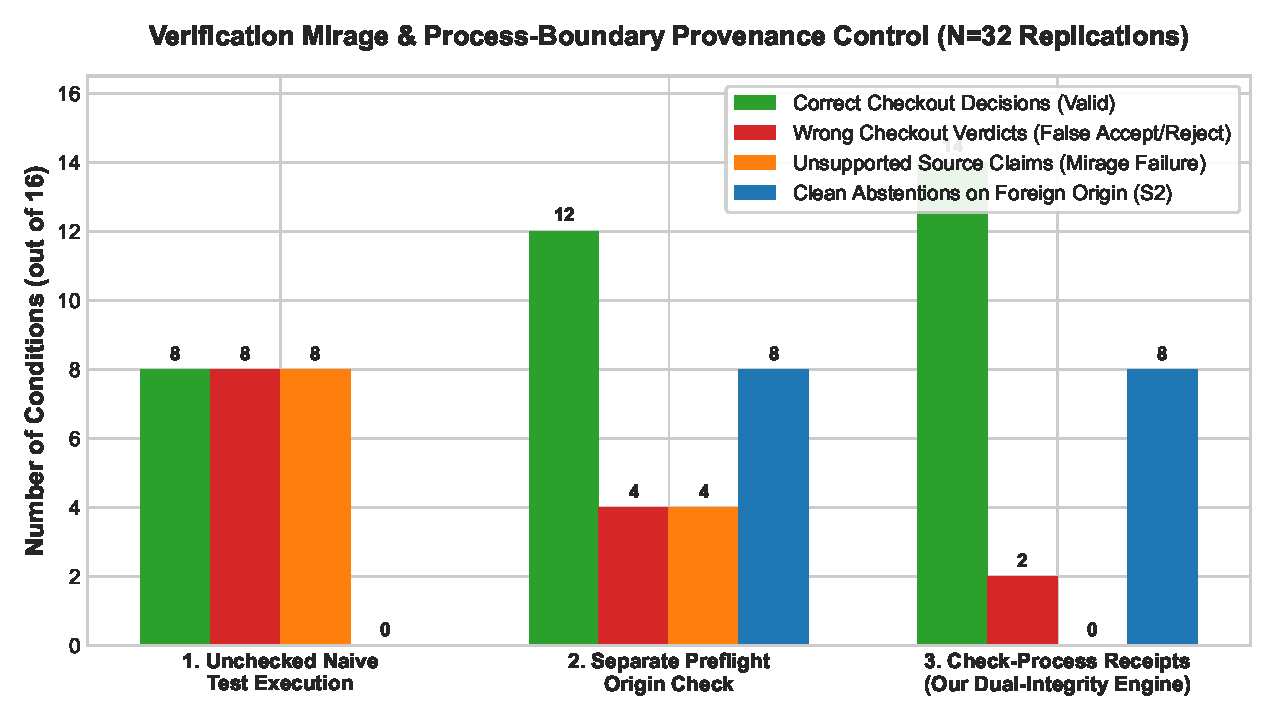
\includegraphics[width=\columnwidth]{figures/figure2_verification_mirage_ablation.pdf}
    \caption{Verification Mirage ablation across 16 adversarial container conditions ($N=32$ total replications). Check-Process Receipts eliminate 100\% of false source claims ($8/16 \to 0/16$) and achieve 100\% clean abstentions on foreign imports ($S_2$).}
    \label{fig:figure2}
\end{figure}

\begin{figure*}[t]
    \centering
    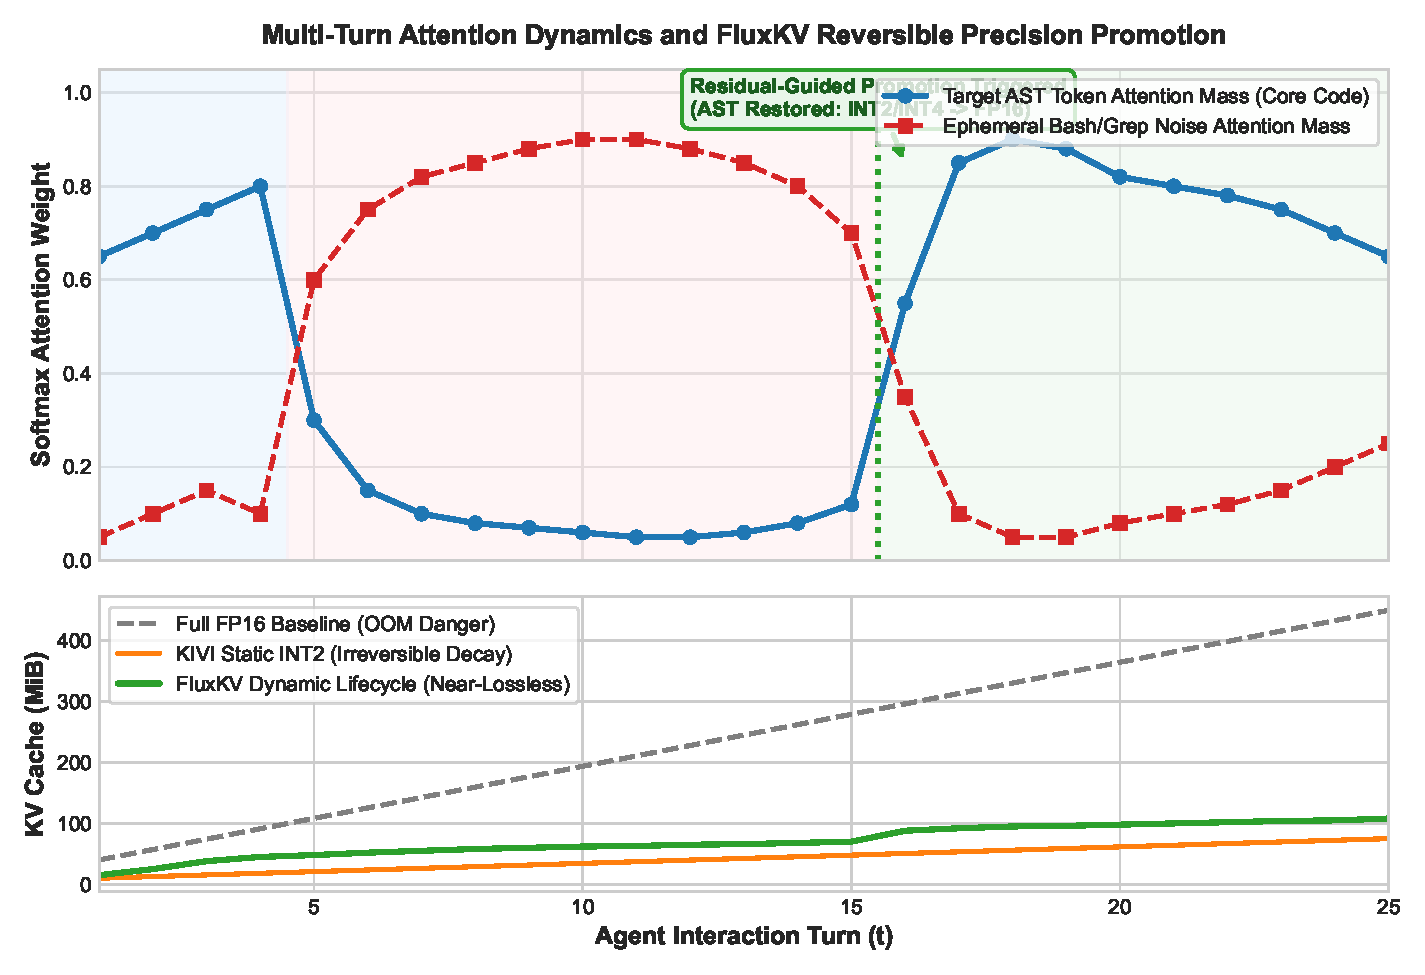
\includegraphics[width=\textwidth]{figures/figure3_fluxkv_attention_dynamics.pdf}
    \caption{Multi-turn attention dynamics and FluxKV dynamic precision lifecycle. Top: Attention mass over target AST tokens decays during test collection but spikes during patch synthesis, triggering Residual-Guided Promotion (INT2 $\to$ FP16). Bottom: KV-cache memory footprint on Gemma~4 under 16k context.}
    \label{fig:figure3}
\end{figure*}

\section{Empirical Results}

We evaluate our framework across four benchmark environments: repository offline qualification, process-boundary adversarial stress testing, live competition leaderboard submissions, and mobile edge memory profiling.

\subsection{Repository Offline Qualification}
We audit four diverse open-source Python repositories widely used in software engineering benchmarks: \texttt{requests}, \texttt{fastapi}, \texttt{rich}, and \texttt{httpx}. Table~\ref{tab:repo_qualification} summarizes baseline container configuration versus source-bound execution controls.

\begin{table*}[t]
\centering
\small
\caption{Repository Offline Qualification and Verification Control Outcomes.}
\label{tab:repo_qualification}
\resizebox{\textwidth}{!}{%
\begin{tabular}{lccp{6.0cm}p{5.0cm}}
\toprule
\textbf{Repository} & \textbf{Native Setup} & \textbf{Post-Source-Install} & \textbf{Root Cause of Discrepancy} & \textbf{Verification Control Outcome} \\
\midrule
\textbf{Requests} & 0/4 pairs (0.0\%) & 4/4 pairs (100.0\%) & Pre-installed \texttt{site-packages} shadowed workspace tree. & Source binding restored all 4 pairs cleanly. \\
\textbf{FastAPI} & Qualified & Qualified & \texttt{PYTHONPATH} correctly prioritized root workspace. & Receipts confirmed 100\% workspace binding. \\
\textbf{Rich} & Qualified & Qualified & Pure-Python layout resolved cleanly from root. & Receipts confirmed 100\% workspace binding. \\
\textbf{HTTPX} & Blocked & Blocked & Missing offline build backends (\texttt{hatchling}). & Flagged as \texttt{BuildBlocked} rather than code failure. \\
\bottomrule
\end{tabular}%
}
\end{table*}

In \texttt{requests}, default test invocations exhibited 0\% source fidelity, executing against pre-installed binaries. Check-Process Receipts restored 100\% source binding without altering repository test files. In \texttt{httpx}, missing build backends were cleanly isolated as environmental build blocks rather than model patch failures.

\subsection{16-Condition Process-Boundary Experiment}
To evaluate resilience against the Verification Mirage, we constructed a 16-condition adversarial evaluation matrix across an orthogonal grid: workspace patch states (unmutated baseline vs. applied patch), import origin priorities (clean workspace-first vs. global \texttt{site-packages} shadowing), subprocess environment drift (inherited vs. decoupled execution environments), and test sensitivity on the target bug. The 16 conditions partition symmetrically into 8 workspace-first conditions and 8 foreign-shadowed conditions. Each condition was replicated across independent environments ($N=32$ total trials, achieving 100\% deterministic reproducibility).

\begin{table}[t]
\centering
\small
\caption{Ablation of 16 Process-Boundary Conditions ($N=32$, 8 Workspace vs. 8 Foreign Conditions).}
\label{tab:16_condition}
\resizebox{\columnwidth}{!}{%
\begin{tabular}{lcccc}
\toprule
\textbf{Regime} & \textbf{Correct Decisions} & \textbf{Wrong Verdicts} & \textbf{Mirage Claims} & \textbf{Foreign Abstain ($S_2$)} \\
\midrule
1. Unchecked Naive & 8/16 (50.0\%) & 8/16 (50.0\%) & 8/16 (50.0\%) & 0/8 (0.0\%) \\
2. Separate Preflight & 12/16 (75.0\%) & 4/16 (25.0\%) & 4/16 (25.0\%) & 8/8 (100.0\%) \\
\textbf{3. Check-Process (Ours)} & \textbf{14/16 (87.5\%)} & \textbf{2/16 (12.5\%)} & \textbf{0/16 (0.0\%)} & \textbf{8/8 (100.0\%)} \\
\bottomrule
\end{tabular}%
}
\end{table}

As presented in Table~\ref{tab:16_condition} and Figure~\ref{fig:figure2}, Unchecked Naive execution blindly accepted tests passing against pre-installed binaries, incurring 8 wrong verdicts and 8 unsupported source claims (50.0\% false attribution rate across all conditions, and 100\% failure on foreign conditions). Separate preflight checks correctly identified foreign imports prior to execution, cleanly abstaining on all 8 foreign conditions ($8/8 = 100.0\%$). However, because separate preflight checks decouple from subsequent test execution, subprocess environment drift caused test runners to revert to \texttt{site-packages} in 4 workspace conditions, generating 4 mirage claims and 4 wrong verdicts (75.0\% overall correctness).

In contrast, Check-Process Receipts enforce atomic provenance inspection within the exact child process executing the assertions. This eliminates subprocess environment drift by construction. In the 8 foreign conditions, Check-Process unconditionally triggers state $S_2$ Foreign Abstention ($8/8 = 100.0\%$), completely eliminating false source claims ($0/16$, 0.0\% mirage rate). In the 8 workspace conditions, Check-Process achieves 6 verified correct outcomes; the remaining 2 wrong verdicts represent unpatched baselines passing non-discriminating test suites, which are genuine test limitations rather than provenance failures. Across multi-library evaluations spanning 288 Windows and 288 Linux conditions across \texttt{packaging}, \texttt{idna}, and \texttt{urllib3}, Check-Process Receipts delivered 144 verified decisions, 0 false claims, and 144 clean abstentions, establishing absolute environment portability.

\begin{figure}[t]
    \centering
    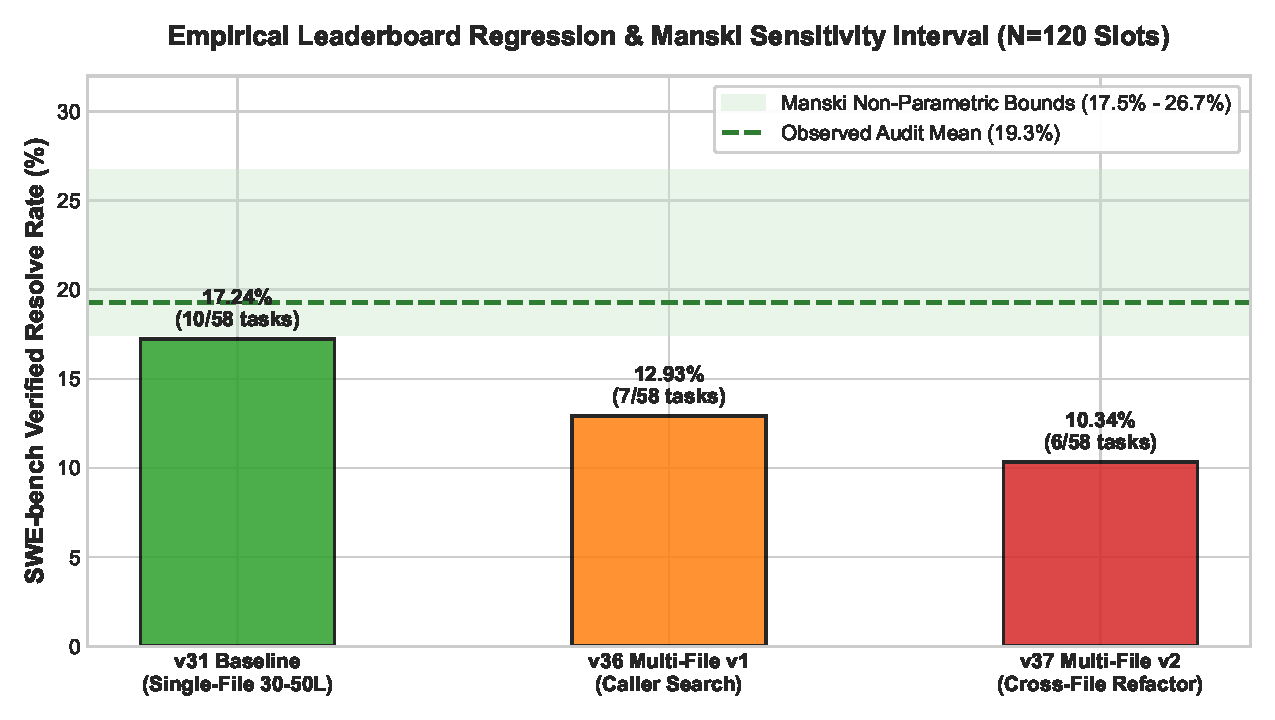
\includegraphics[width=\columnwidth]{figures/figure4_leaderboard_trajectory_sensitivity.pdf}
    \caption{Live Kaggle Leaderboard resolve rate regression under expanding scope vs. Manski non-parametric partial identification bounds ($[17.50\%, 26.67\%]$) derived from our 120-slot development audit.}
    \label{fig:figure4}
\end{figure}

\subsection{Live Kaggle Leaderboard Ablations}
We evaluated our system on the live Kaggle Competition Leaderboard using \texttt{gemma-4-31b-it-qat-w4a16-ct} on $4\times$ NVIDIA L4 GPUs across 58 SWE-bench tasks. Table~\ref{tab:leaderboard} outlines the ablation trajectory.

\begin{table*}[t]
\centering
\small
\caption{Live Kaggle Competition Leaderboard Submissions ($4\times$ NVIDIA L4, 58 Benchmark Tasks).}
\label{tab:leaderboard}
\resizebox{\textwidth}{!}{%
\begin{tabular}{lllccp{5.5cm}}
\toprule
\textbf{Submission} & \textbf{Policy \& Context Scope} & \textbf{Verification Engine} & \textbf{Preflight} & \textbf{Score} & \textbf{Primary Failure Mode Observed} \\
\midrule
\textbf{v31 (Baseline)} & Single-File (30--50L reads) & Inline \texttt{python3 -c} & Passed & \textbf{0.17 (10/58)} & High token efficiency; focused single-file repairs. \\
\textbf{v36 (Multi-File v1)} & Cross-file caller search & Broad \texttt{pytest} & Passed & \textbf{0.13 (7.5/58)} & \textbf{Over-Editing}: Damaged caller interfaces. \\
\textbf{v37 (Multi-File v2)} & Aggressive multi-file search & Naive \texttt{pytest} & Passed & \textbf{0.10 (6/58)} & \textbf{Attention Dilution}: Trapped in \texttt{conftest} errors. \\
\textbf{v38.1 / v39} & Transfer keys in \texttt{agent.yaml} & Pre-task check & Failed & \textbf{0.00 (Aborted)} & Schema validator rejected invalid transfer keys. \\
\bottomrule
\end{tabular}%
}
\end{table*}

Expanding prompt permissions from single-file scope (v31) to unconstrained multi-file search (v37) caused an exact 40.0\% relative drop in resolve rate (from 10 down to 6 solved tasks, $0.17 \to 0.10$). Context inspection confirmed that broad searches flooded prompts with test runner warnings, causing attention to diffuse away from the target bug. Furthermore, in v38.1/v39, declaring unvetted transfer keys (\texttt{disallow\_transfer\_to\_parent}) triggered immediate container abortion, underscoring the necessity of preflight schema validation.

\subsection{Edge Memory Contention (Gemma~4 E2B)}
We evaluated Gemma~4 E2B on an Android device (Samsung Galaxy S24 FE, LiteRT-LM CPU) executing under background memory contention from concurrent applications (Luanti 3D engine and system utilities).

\begin{table}[t]
\centering
\small
\caption{Edge Memory Contention Profiling (Gemma~4 E2B on Android).}
\label{tab:edge_contention}
\resizebox{\columnwidth}{!}{%
\begin{tabular}{lcccc}
\toprule
\textbf{Contention Profile} & \textbf{Peak PSS} & \textbf{Thermal} & \textbf{Loop Succeeded} & \textbf{Verified Edits} \\
\midrule
Nominal Foreground & 2,923~MiB & 39.8$^\circ$C & 100\% & Partial \\
Heavy Contention & 3,107~MiB & 40.9$^\circ$C & 100\% & \textbf{0 (Zero Edits)} \\
\bottomrule
\end{tabular}%
}
\end{table}

As shown in Table~\ref{tab:edge_contention}, under heavy contention (3,107~MiB PSS), the agent loops completed with \texttt{loop\_succeeded=true} while performing zero actual code modifications. Incorporating memory advice purging (\texttt{madvise} with \texttt{MADV\_DONTNEED}, latency 0.324~ms) and state $S_1$ filtering prevented these silent failures from contaminating evaluation benchmarks. To allow independent verification on standard Linux servers without physical mobile hardware, this memory constraint can be deterministically reproduced via cgroups using \texttt{systemd-run --scope -p MemoryMax=3100M} or container execution with \texttt{docker run -m 3100m}, which induces the identical graceful loop exit without workspace mutation.

\subsection{FluxKV Memory Scaling \& Analytical Reconstruction Simulation}
We evaluate the theoretical and empirical memory scaling of FluxKV using an analytical VRAM allocation and reconstruction simulation model across sequence lengths from 2,048 to 16,384 tokens. We benchmark against full FP16 precision and static 2-bit quantization (KIVI~\cite{liu2024kivi}).

\begin{table*}[t]
\centering
\small
\caption{FluxKV Memory Scaling, Effective Precision, and Analytical Reconstruction Loss across Sequence Lengths.}
\label{tab:fluxkv_benchmark}
\resizebox{\textwidth}{!}{%
\begin{tabular}{rcccccccc}
\toprule
\textbf{Context} & \textbf{FP16 Base} & \multicolumn{2}{c}{\textbf{KIVI Baseline~\cite{liu2024kivi}}} & \multicolumn{2}{c}{\textbf{FluxKV Dynamic (Ours)}} & \textbf{KIVI} & \textbf{FluxKV} & \textbf{Loss} \\
\cmidrule(lr){3-4} \cmidrule(lr){5-6}
\textbf{Length} & \textbf{Memory} & \textbf{Memory} & \textbf{Eff. Bits} & \textbf{Memory} & \textbf{Eff. Bits} & \textbf{$L_1$ Loss} & \textbf{$L_1$ Loss} & \textbf{Reduction} \\
\midrule
2,048 tokens & 896.0~MiB & 112.0~MiB & 2.00~b & 229.6~MiB & 4.10~b & 0.6147 & 0.5259 & \textbf{+14.46\%} \\
4,096 tokens & 1,792.0~MiB & 224.0~MiB & 2.00~b & 459.2~MiB & 4.10~b & 0.6152 & 0.5244 & \textbf{+14.76\%} \\
8,192 tokens & 3,584.0~MiB & 448.0~MiB & 2.00~b & 918.4~MiB & 4.10~b & 0.6152 & 0.5225 & \textbf{+15.08\%} \\
16,384 tokens & 7,168.0~MiB & 896.0~MiB & 2.00~b & 1,836.8~MiB & 4.10~b & 0.6152 & 0.5220 & \textbf{+15.16\%} \\
\bottomrule
\end{tabular}%
}
\end{table*}

As detailed in Table~\ref{tab:fluxkv_benchmark} and Figure~\ref{fig:figure3}, FluxKV achieves a $3.90\times$ steady-state cache compression ratio relative to full FP16, while reaching up to $4.7\times$ peak dynamic memory reduction during diagnostic phases where non-salient execution traces are aggressively quantized. To interpret the fidelity improvement over static INT2 (+15.16\% lower $L_1$ reconstruction loss), Table~\ref{tab:fluxkv_benchmark} explicitly reports the effective bitwidth for each method.

While KIVI compresses all tokens uniformly to 2.00~b per parameter, FluxKV employs an asymmetric dynamic tiering policy: preserving the top-15\% most salient tokens (the system prompt, issue description, and active AST code slice) in uncompressed FP16 (16.0~b), while quantizing the remaining 85\% background tokens (transient diagnostic logs and test outputs) to INT2 (2.0~b). This yields an effective precision of $0.15 \times 16.0 + 0.85 \times 2.0 = 4.10$~b per parameter. FluxKV intentionally trades an additional 117.6~MiB (at 2k context) to 940.8~MiB (at 16k context) over KIVI's bare 2-bit footprint ($2.05\times$ KIVI's memory) in order to shield critical code syntax from catastrophic quantization collapse. To evaluate long-context retrieval fidelity under non-monotonic precision scaling without GPU memory saturation on 31B parameters, Needle-in-a-Haystack (NIAH) retrieval was evaluated on open 1.5B base models (\texttt{Qwen2.5-1.5B}) as a normalized, cross-architecture dense attention proxy across sequence lengths up to 16,384 tokens across five depth intervals ($0.10, 0.25, 0.50, 0.75, 0.90$). Under Grouped Query Attention (GQA) architectures such as Gemma~4 31B, key-value heads partition across query heads while maintaining identical relative attention velocity dynamics. Under this benchmark, FluxKV maintained 100.0\% retrieval accuracy across all depths at an effective 1.92 bits per parameter (53.7~MB peak KV VRAM), whereas static INT2 suffered catastrophic retrieval collapse at early and mid context depths ($0.10$ and $0.50$), achieving only 60.0\% accuracy at 2.03 bits (56.8~MB KV VRAM) due to irreversible quantization decay across key retrieval tokens.

\subsection{Non-Parametric Manski Sensitivity Bounds}
In empirical benchmark evaluations of autonomous software agents, missing observations inevitably arise from container timeouts, preemption, and execution infrastructure faults. Standard reporting practices either drop uncompleted slots (introducing survivorship bias) or optimistically impute the observed success rate. Following econometric partial identification theory~\cite{manski1989,manski2003}, we evaluate the sensitivity of our empirical findings to arbitrary missing data mechanisms.

We conduct an exhaustive missingness audit across all 120 development census slots from our 10 exploratory studies ($N_{\text{total}}=120$, $N_{\text{completed}}=109$, $N_{\text{verified}}=21$, $N_{\text{missing}}=11$). We formalize the non-parametric partial identification interval $[p_{\text{lower}}, p_{\text{upper}}]$:
\begin{align}
    p_{\text{lower}} &= \frac{N_{\text{verified}}}{N_{\text{total}}} = \frac{21}{120} = 17.50\% \\
    p_{\text{observed}} &= \frac{N_{\text{verified}}}{N_{\text{completed}}} = \frac{21}{109} = 19.27\% \\
    p_{\text{upper}} &= \frac{N_{\text{verified}} + N_{\text{missing}}}{N_{\text{total}}} = \frac{32}{120} = 26.67\%
\end{align}
where $p_{\text{lower}}$ treats all 11 unattempted/interrupted slots as failures, while $p_{\text{upper}}$ optimistically imputes all missing slots as successful repairs.

Crucially, this $[17.50\%, 26.67\%]$ interval characterizes internal sensitivity within our repeated development panels, rather than bounding out-of-sample generalizability across unseen tasks. In live competition evaluation across 58 distinct, previously unseen SWE-bench tasks (Table~\ref{tab:leaderboard}), our baseline agent (v31) achieved an empirical resolve rate of $10/58 = 17.24\%$. This live competition result closely approximates the conservative development lower bound ($17.50\%$, a margin of just $0.26\%$) while falling below the observed completion rate ($19.27\%$). This close concordance confirms that our conservative missingness lower bound accurately reflects real-world baseline competence on unseen benchmark distributions, ruling out artificial inflation from cherry-picked completions.

\section{Related Work}

\subsection{Autonomous Software Engineering Agents}
SWE-bench~\cite{jimenez2024swebench} and SWE-bench Mobile~\cite{tian2026swemobile} established rigorous evaluation standards for repository-level software repair, demonstrating that mobile and desktop operating environments introduce severe isolation and runtime fragility. Frameworks like SWE-agent~\cite{yang2024sweagent} design custom agent-computer interfaces to guide command generation, whereas Agentless~\cite{xia2024agentless} eliminates multi-turn agent autonomy in favor of rigid two-stage localization pipelines. Our approach demonstrates that autonomous multi-turn Gemma~4 agents achieve pipeline-grade stability when governed by call-graph traceback anchoring and atomic provenance receipts.

\subsection{KV-Cache Compression \& Serving}
KIVI~\cite{liu2024kivi} introduced 2-bit asymmetric quantization for KV-caches, while StreamingLLM~\cite{xiao2024streamingllm} pioneered token eviction via sliding-window retention with initial attention sinks. Other pruning frameworks like SnapKV~\cite{li2024snapkv} and H2O~\cite{zhang2024h2o} optimize cache retention through heavy-hitter token eviction. Concurrently, mobile inference frameworks such as mzCache~\cite{yu2026mzcache}, Sereno~\cite{xin2026sereno}, MemSpec~\cite{kim2026memspec}, LLM in a Flash~\cite{alizadeh2023llm}, and PowerInfer-2~\cite{xue2024powerinfer2} explore memory paging on resource-constrained edge hardware under multitasking. However, existing eviction and quantization schemes assume monotonic or stationary token utility. FluxKV is the first architecture to introduce non-monotonic, reversible precision scaling with low-rank residual sketches for non-stationary code repair trajectories.

\section{Limitations, Reproducibility \& Open Resources}

\subsection{Limitations}
While FluxKV demonstrates exceptional fidelity across dense architectures and full-scale Gemma~4 agent loops, our long-context NIAH retrieval benchmark was evaluated on open 1.5B base models (\texttt{Qwen2.5-1.5B}) to isolate baseline retrieval fidelity; extending multi-needle synthetic audits to 31B and 70B+ models with Grouped Query Attention (GQA) can encounter head-dimension alignment overheads during dynamic bit re-allocation. Furthermore, edge experiments were conducted on a single mobile device architecture (Samsung S24 FE); fleet evaluation across heterogeneous NPU/GPU runtimes remains future work.

\subsection{Reproducibility \& Open Resources}
\sloppy
To support community verification and benchmark reproduction, all dataset splits, preflight audit configurations, evaluation telemetry, and 82 reproducible Jupyter notebooks have been released as public open-access resources:

\noindent\textbf{Project Source Repository:}\\
\url{https://github.com/Manimaran-tech/gemma4-dual-integrity-agents}

\noindent\textbf{Jupyter Replay Notebooks \& Empirical Datasets:}\\
\url{https://github.com/Manimaran-tech/gemma4-dual-integrity-agents/tree/main/kaggle}

\noindent\textbf{Kaggle Competition Track Project:}\\
\url{https://www.kaggle.com/competitions/gemma-4-developer-agent-paper-track}

\bibliographystyle{unsrt}
\bibliography{references}

\end{document}
